\documentclass{article}
\usepackage{settings}


\date{\today}

\begin{document}
\thispagestyle{empty}
\begin{center}
    \LARGE\textbf{МИНОБРНАУКИ РОССИИ\\
        САНКТ-ПЕТЕРБУРГСКИЙ ГОСУДАРСТВЕННЫЙ\\
        ЭЛЕКТРОТЕХНИЧЕСКИЙ УНИВЕРСИТЕТ\\
        "ЛЭТИ"\ ИМ. В.И.УЛЬЯНОВА(ЛЕНИНА)\\
        Кафедра МО ЭВМ}\\[4cm]
    \Large\textbf{ОТЧЁТ}\\[0.2cm]
    \Large\textbf{по лабораторной работе}\\[0.1cm]
    \Large\textbf{по дисциплине <<Базы данных>>}\\[0.1cm]
    \Large\textbf{Тема: <<Проектирование ER модели и структуры БД по текстовому описанию предметной области>>.}\\[3cm]
\end{center}
\Large{Студент гр. 1304 \qquad \qquad \quad \underline{\hspace{6cm}} \qquad \qquad Мусаев А.И.}\\[0.5cm]
\Large{Преподаватель \qquad \qquad \qquad \underline{\hspace{6cm}} \qquad \qquad Заславский М.М.}\\[1cm]
\begin{center}
    Санкт-Петербург\\
    2023
\end{center}
\newpage

\textbf{Цель работы}

Проектирование ER модели и структуры БД по текстовому описанию предметной области.

\textbf{Задание}

Вариант - 16.

Пусть требуется создать программную систему, предназначенную для врачей и работников регистратуры поликлиники. Такая система должна хранить сведения об участках, которые относятся к поликлинике, о расписании работы участковых врачей, информацию о врачах, а также карточки пациентов. Карточка имеет номер, в нее заносятся сведения о каждом посещении поликлиники пациентом: дата посещения, жалобы, предварительный диагноз, назначения, выписан или нет больничный лист, и, если выписан, то на какой срок, имя врача. В карточке на первой странице указаны также фамилия, имя, отчество пациента, его домашний адрес, пол и возраст, номер страхового полиса, дата заполнения карточки. В расписании работы врачей указывается, на каком участке работает врач, дни и часы приема, номер кабинета. Врач может обслуживать более одного участка. В случае увольнения врача его участок(участки)передается другим врачам. Данные о враче, которые хранятся в БД, - это фамилия, имя отчество, категория, стаж работы, дата рождения. В карточку больного при каждом его посещении поликлиники врачом заносится очередная запись. Работники регистратуры регистрируют пациента, заполняя первую страницу его карточки. Уволить врача имеет право только заведующий поликлиникой. Он удаляет из базы сведения о враче и передает его больных другому врачу.

\begin{itemize}
    \item Выбрать вариант задания: ((N - 1) mod M ) + 1, где N - номер в группе, M - число вариантов (22), нумерация с 1. То есть если вы в списке 1, то берете 1, 22 - 22, 23 - 1.
    \item  Нарисовать ER модель, рекомендуется использовать draw.io или иной редактор
    \item Нарисовать ER модель, рекомендуется использовать draw.io или иной редактор
    \item Нарисовать структуру БД, содержащую названия полей, таблиц, связи, типы данных, ключи.
    \item Проверить и обосновать, что реляционная модель соответвует НФБК
    \item Прикрепить 2 изображения (er.png, db.png) в PR
    \item Описать полученные модели, для чего нужна каждая сущность, почему такие связи и т.п.
    \item В отчете описать цель, текст задания в соответствии с вариантом, 2 изображения моделей, их описание, обоснование НФБК, ссылку на PR в приложении, вывод

\end{itemize}

\textbf{Выполнение работы}

ER-модель и структура базы данных представлена в приложении.

В структуре БД использованы следующие сущности:

\begin{enumerate}
    \item Пациент (Patient)

    Атрибуты: номер карточки (patientID, PK), фамилия (surname), имя (name), отчество (patronymic), адрес (adress), пол (sex), возраст (age), дата создания карточки (dateCreating).
    
    \item Посещение (Visit)

    Атрибуты: дата (date), диагноз (diagnosis), рекомендации (appointments), жалобы (complaints), дано ли освобождение (givenLeave), срок (term), номер доктора (doctorID), номера карты пациента (patientCardID).

    \item Доктор (Doctor)

    Атрибуты: номер доктора (doctorID), фамилия (surname), имя (name), отчество (patronymic), специализация (category), дата рождения (birthDate), расписание доктора (doctorSchedule), номер клиники (clinicID).

    \item Расписание доктора (DoctorSchedule)

    Атрибуты: время посещения (receptionTime), кабинет (cabinet), название района (nameArea), номер доктора, обслуживающего этот участок (doctorID).

    \item Участок клиники (selectionClinic)

    Атрибуты: номер района (nameArea), название клиники (title).

    \item Поликлинника (Clinic)

    Атрибуты: название (title).
\end{enumerate}

Доказательство, что модель соответствует НФБК:

1NF:

- В таблице нет дублирующих строк

- В каждой ячейке хранится атомарное значение

- В столбце хранятся данные одного типа

- Отсутствуют массивы и списки

2NF:

- У таблиц есть ключ

- Все неключевые столбцы зависят от полного ключа

3NF:

- В таблицах нет транзитивной зависимости

\newpage

\textbf{Вывод}

Были спроектированы ER модель и структура БД по текстовому описанию предметной области.

\newpage

\centerline{\textbf{Приложение A}}

\href{https://github.com/moevm/sql-2023-1304/pull/4}{Ссылка на PR (кликабельна)}

\centerline{\textbf{Приложение B}}

\begin{figure}[h]
\centering
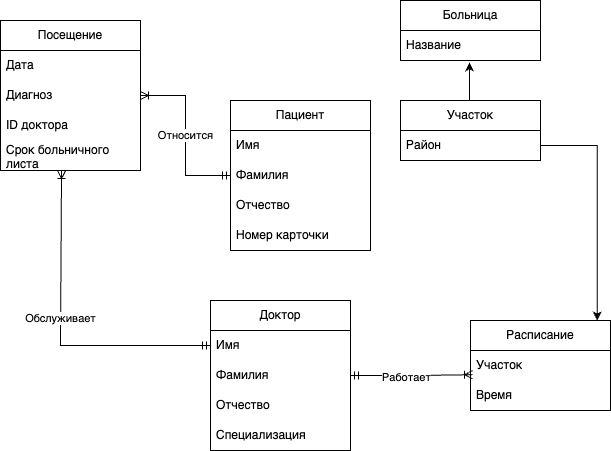
\includegraphics[width=1\linewidth]{er.png}
\caption{Er-модель}
\label{fig:mpr}
\end{figure}

\newpage

\centerline{\textbf{Приложение C}}

\begin{figure}[h]
\centering
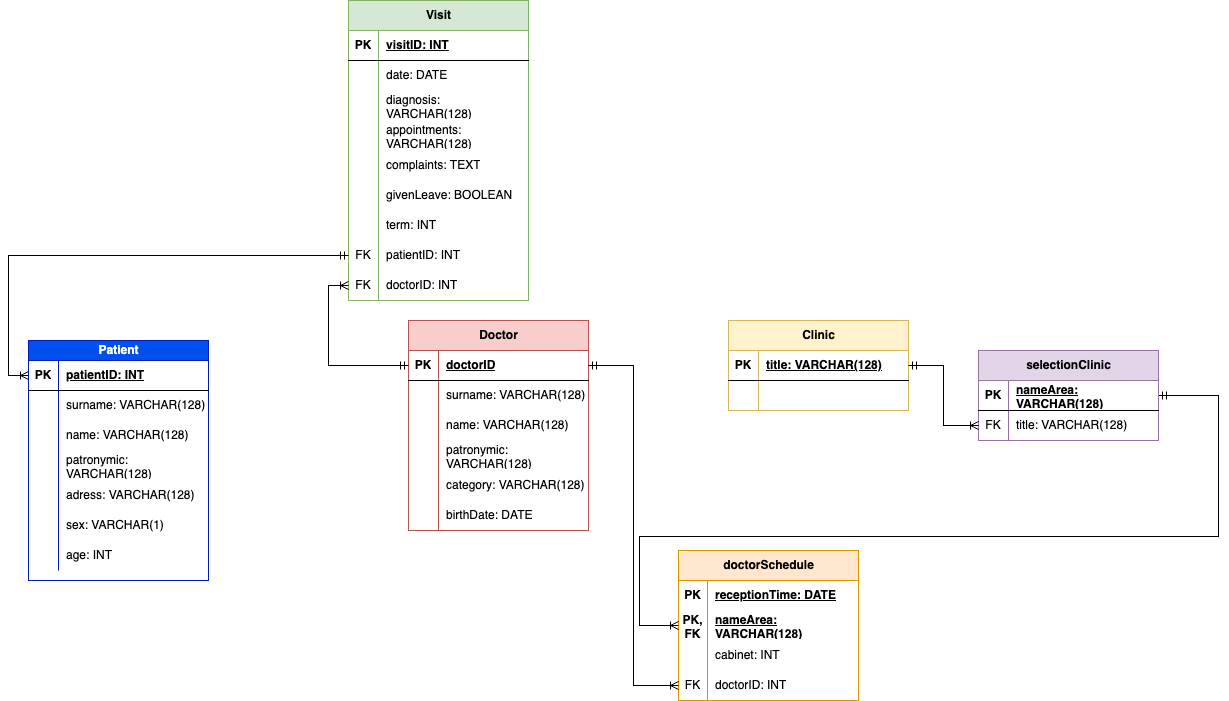
\includegraphics[width=0.95\linewidth]{bd.png}
\caption{Структура БД}
\label{fig:mpr}
\end{figure}

\end{document}